\definecolor{ribbon}{HTML}{E0E0E0}

My alternative approach to co-optation and political
repression probes their interaction more
directly.\footnote{For detailed results see Appendix B.} I
assume that the attenuating effect of co-optation on
empowerment rights restrictions that Erica Frantz and Andrea
Kendall-Taylor discuss is conditional on the level of
physical integrity violations. The more dictators engage in
torture and mayhem, the less credible become their
institutional commitments. Thus, I assume that the extent of
physical integrity violations undermines any supporting
effect that political parties and legislatures might have
on the validity of empowerment rights. To ascertain the
validity of this intuition I apply an ordinary least
squares regression to the unimputed raw data. As this
extension serves as a first approximation to a more  general
research project I forego multiple imputation and  focus on
more pressing concerns of variable selection,  statistical
design, and validation.

Frantz' and Kendall-Taylor's analyses include numerous 
predictors that are not meaningful control variables. For 
instance, trade in per cent of GDP per capita 
neither correlates with political repression nor with 
co-optation. Thus, as a first design decision I remove all
variables from the analysis that have a Pearson's $|r|$ of 
less than $0.1$ with any of the three core variables. 
Second, I employ co-optation as a categorical predictor to
validate the original coding scheme. Third, I replace Beck's 
and Katz's standard TSCS recipe with the default 
heteroskedasticity and autocorrelation consistent covariance
estimator described by \citet[6]{Zeileis.2004}. Fourth, I 
focus on the $t+1$ formulation of empowerment 
rights. Finally, I use 28 of 133 countries in the data as a 
validation set for the extended model in order to probe its 
external validity \cite[175ff.]{James.2013}.

\begin{figure}[!htb]
  \centering
  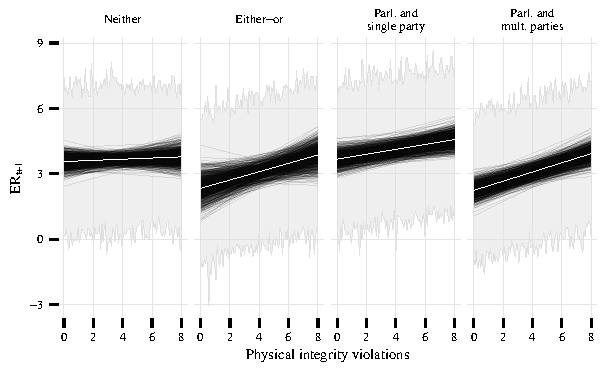
\includegraphics[width = \linewidth]{./sections/04extension/spaghettiInteraction.pdf}
  \caption{Simulated interaction of co-optation and physical integrity violations}
  \label{fig:simInteraction}
\end{figure}

Although most of the basic terms are not statistically 
significant an analysis of variance and a likelihood ratio 
test both find the assumed interaction to improve model fit.
Using simulations with $1,000$ iterations 
Figure \ref{fig:simInteraction} evaluates 
it in more detail 
\citep{KingGaryMichaelTomzWittenbergJason.2000}. Ribbons in 
each panel denote stochastic 
uncertainty ({\color{ribbon} $\bullet$}) and faded lines
represent systematic uncertainty ($\bullet$). White lines 
average over all estimates of systematic uncertainty and 
denote a mean effect. Figure \ref{fig:simInteraction} shows 
that empowerment rights restrictions at $t+1$ increase in 
physical integrity violations for all but the `Neither' 
category of co-optation. Furthermore, the intercepts of the 
mean effect graphs do \textit{not} systematically decrease 
when moving from the `Neither' to the `Multi-party 
legislature' category of the co-optation index. Finally, 
ranges of systematic and stochastic uncertainty overlap 
between all panels. Taken together these observations on
Figure \ref{fig:simInteraction} establish three crucial 
results: 1. The existence of political parties and 
parliaments does not lend itself to a linear additive index 
of co-optation; 2. Increasing physical integrity violations 
concur with increasing restrictions on empowerment rights 
under almost all institutional settings; 3. This finding 
seems not to be substantially significant.

Although the preceding analysis dampens optimistic 
expectations the extended model might still generalize 
meaningfully to other contexts. After all, 
simulations are a very tough benchmark for every statistical
model. However, when moving to the validation-set my 
attempted extension fails again. For instance, the root mean
square error (RMSE) of the training set is $1.01$. It  
improves considerably over the standard deviation of the 
dependent variable in the training set ($1.24$). 
Nonetheless, the test-set RMSE is $1.49$ -- an almost 50 
per cent increase over the training set. More importantly, 
the fitted model systematically overestimates within-country
variation in the validation sample. This can be seen from 
the slope plot in Figure \ref{fig:testSample}, which 
compares within-country standard deviations in empowerment 
rights restrictions at $t+1$ to the corresponding 
within-country RMSE. Special emphasis is given to Saudi 
Arabia and Georgia which have the largest respectively 
smallest RMSE. Very few lines exhibit a negative slope or 
are at least constant as in the case of Georgia. Clearly 
dominant is the impression of an upward trend in 
within-country variation, which can be as large as a 
fivefold increase. This is the case in Saudi Arabia. In 
short, the assumed interaction does not generalize beyond 
the training set.

\begin{figure}[!htb]
  \centering
  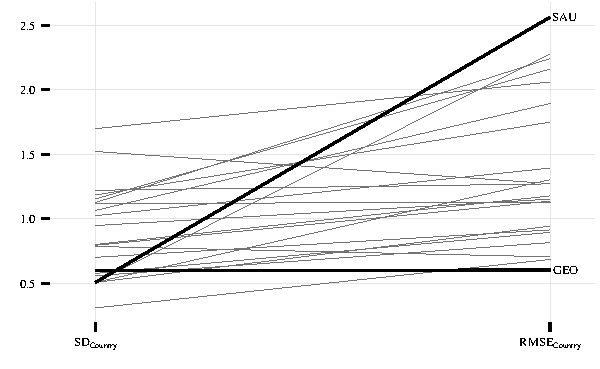
\includegraphics[width = \linewidth]{./sections/04extension/testSamplePred.pdf}
  \caption{Country-based out-of-sample performance}
  \label{fig:testSample}
\end{figure}

To summarize, despite its statistical significance the 
assumed interaction of co-optation and physical integrity 
violations is neither substantially significant nor
externally valid. Moreover, it is apparent from the 
preceding analysis that the existence of political parties 
and legislatures does not lend itself to a linearly additive
index of co-optation. Finally, my simple ordinary 
least-squares regression overestimates within-country 
variation in empowerment rights restrictions because it 
cannot separate lateral from longitudinal variance. In 
short, the analysis of co-optation and political repression 
in authoritarian regimes requires better measurements and 
more sophisticated statistical designs.